\section{电磁继电器}\label{sec:10-6}

人们直接去操纵高电压、强电流的开关是很危险的。怎么办呢?
利用电磁铁做成的电磁继电器可以帮助我们解决这个问题。
图 \ref{fig:10-30} 所示的是利用电磁继电器控制电动机的电路。
由电磁铁、低压电源和电键组成控制电路。
由电动机、高压电源和电磁继电器的触点部分组成工作电路。
\begin{figure}[htbp]
    \centering
    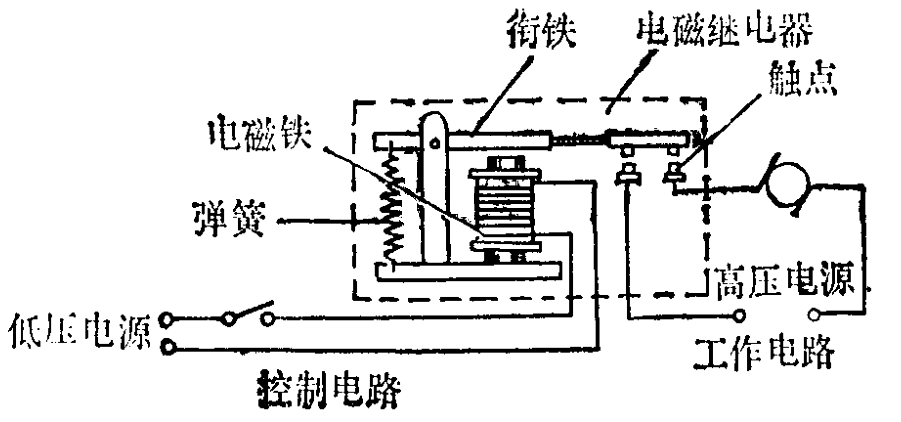
\includegraphics[width=0.6\textwidth]{../pic/czwl2-ch10-30}
    \caption{电磁继电器工作原理}\label{fig:10-30}
\end{figure}
合上电键, 电磁铁线圈中有微弱的控制电流通过时,电磁铁就吸引衔铁,使工作电路闭合,电动机启动。
把控制电路的电键断开,电磁铁线圈中没有控制电流时,弹簧就把衔铁拉起,切断了工作电路,电动机就停止工作。
这个例子告诉我们利用电磁继电器可以用低电压、弱电流控制高电压、强电流的工作电路。

利用电磁继电器还可以实现远距离操纵和自动控制,这给人们的工作带来不少方便。
把控制电路的电键安装在离工作地点很远的操作方便的地方,把电磁继电器安装在工作地方,就可以实现远距离操纵。
至于用电磁继电器来实现自动控制,同学们在做过练习三的习题后,就可以有所体会。

